This section of the report discusses the developement of the Optika package.

\section{Initial Planning}
In Fall of 2008. Dr. Mike Heroux identified a need for
the Trilinos framework to include some sort of GUI package. Dr. Heroux wanted 
to give users of the framework the ability to easily generate GUIs for their
programs, while still providing a good experience for the end user. Based on
previous GUI work done for the Tramonto project, a few initial problems were
identified:

	\begin{itemize}
		\item How would the GUI be laid out?
		\item Different types of parameters require different methods of input.
			How would we decide how we would obtain input for a particular
			parameter?
		\item What framework would we use to build the GUI?
		\item How would the application developer specify parameters for the
			GUI to obtain?
		\item How would the application developer specify dependencies between
		parameters. This was a crucial problem/needed feature that was identified in
		development of the Tramonto GUI.
	\end{itemize}

After some deliberation, the following initial solutions were decided upon:

	\begin{itemize}
		\item The GUI would be laid out in a hierarchical fashion as shown in
		Figure \ref{paramlistFigure}. Parameters organized into lists and sublists. This
		would allow for a clear organization of the parameters as well as
		intrinsically demonstrate the relationships between them.
		\begin{figure}
			\centering
			\begin{picture}(50,150)(0,0)
				\put(10,0){\line(0,1){145}}
				\put(0,150){${Parameter List}$}
				\put(10,130){\line(1,0){15}}
				\put(28,127){$Parameter$}
				\put(10,110){\line(1,0){15}}
				\put(28,107){$Parameter$}
				\put(10,90){\line(1,0){15}}
				\put(28,87){$Parameter$}
				\put(10,70){\line(1,0){15}}
				\put(28,67){$Parameter List$}
				\put(38,0){\line(0,1){62}}
				\put(38,47){\line(1,0){15}}
				\put(56,44){$Parameter$}
				\put(38,22){\line(1,0){15}}
				\put(56,24){$Parameter$}
			\end{picture}
			\caption[GUI Layout]{The hierarchical layout of the GUI}
			\label{paramlistFigure}
		\end{figure}
		\item It be required that all parameters specify their type and the
		following types would be accepted:
			\begin{itemize}
				\item int
				\item short
				\item float
				\item double
				\item string
				\item boolean
				\item arrays of int, short, double, and string
			\end{itemize}
		For number types, a spin box would be used as input. If the valid
		values for a string type were specified, a combo box would be used.
		Otherwise a line edit would be used. For booleans, a combo box would
		also be used. For arrays, a pop-up box containing numerous input
		widgets would be used. The widget type would be determined by the
		array type.
		\begin{figure}[h]
			\centering
			\subfigure[A Spin Box]{
				\label{spinboxfig}
				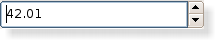
\includegraphics{graphics/spinbox}
			}
			\subfigure[A Combo Box]{
				\label{comboboxfig}
				
\includegraphics{graphics/combobox}
			}
			\subfigure[A Line Edit]{
				\label{lineeditfig}
				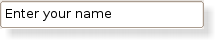
\includegraphics{graphics/lineedit}
			}
			\caption{Some of the various widgets used for editing data}
			\label{editingWidgets}
		\end{figure}

		\item QT was chosen as the GUI framework for several reasons:
			\begin{itemize}
				\item It is cross-platform.
				\item It is mature and has a well developed set of
				development tools.
				\item It has a rich feature-set.
				\item It has been used by Sandia in the past.
				\item The Optika developer was familiar with it.
			\end{itemize}
		\item Initially it was decided that the application developer would
		specify parameters via an XML file. A DTD would be created specifying
		the legal tags and name spaces.
		\item Dependencies would be handled through special tags in the DTD.
	\end{itemize}

\section{Early Development}
The first several months of development were spent on creating and implementing the XML
specification. The name of the XML specification went through several revisions but was
eventually called Dependent Parameter Markup Language (DPML).

After several months of development it was realized that creating an entirely new way of specifying 
parameters might hinder it's adoption. It pointed out that Trilinos actually had
a ParameterList~\cite{ParameterList} class in the Teuchos package. The ParameterList semmed to be better than DPML for
several reasons:
	\begin{itemize}
		\item It was already heavily adopted.
		\item It had the necessary hierarchical nature.
		\item It was serializable to and from XML.
	\end{itemize}

For these reasons, DPML was scrapted in favor of using Teucho's ParameterLists. Development moved
forward with the goal of creating a GUI framework that, in addiiton to meeting all the challenges 
outlined above, would also be compatiable with any existing program using Teuchos's ParameterLists.

\section{Heavy development}
Starting in May 2009 a more heavy focus was put on developement of the Trilinos GUI package.
With the backend data-structure of the Teuchos's ParameterList already in place, attention
was turned to the developing the actually GUI itself. A key technology provided by Qt was it's Model/View
framework~\cite{QtModelView}. Using the Model/View paradigm, a wrapper class named TreeModel
~\cite{TreeModel} was created around the ParameterList class by subclassing the 
QAbstractItemModel~\cite{QAbstractItemModel}.

However, in subclassing the QAbstractItemModel it was realized that the ParameterList class fell short in
certain areas. At this point the main issue was that a given ParameterEntry~\cite{ParameterEntry} located within
a ParameterList or a given sublist located within a ParameterList was not aware of it's parent.
This was an issue because Qt's Model/Veiw framework requires items within a model to be aware of
their parents. In order to circumvent this issue the TreeItem~\cite{TreeItem} class was created. Now 
instead of simply wrapping around a ParameterList class, the TreeModel created by giving it a ParameterList.
It would then read in the ParameterList and creat a structure of TreeItems.  Each TreeItem then contained a pointer 
to it's corresponding ParameterEntry.

Once the TreeModel and TreeItem class were complete an appropriate delegate to go between and View
and the TreeModel was needed. A new class called Delegate~\cite{Delegate} was created to fill this
role by subclassing QItemDelegate~\cite{QItemDelegate}. As specified above, the delegate would return
the apporiate editing widget based on it's datatype.

With the model and delegate classes inplace, an appropriate view could be applied. At first a simple
QTreeView~\cite{QTreeView} was applied to the model. The results was something like that in \ref{treeviewFig}.
	\begin{figure}
		\centering
		\label{treeviewFig}
		\caption[A simple Tree View]
		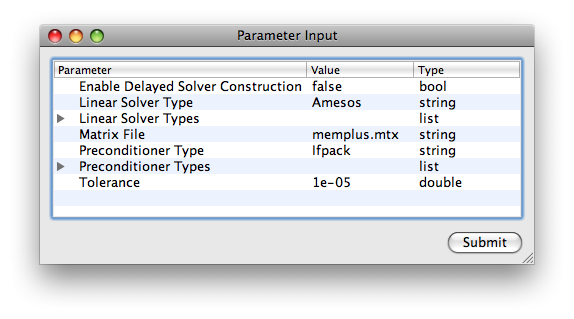
\includegraphics{graphics/treeview}
	\end{figure}


